\documentclass[]{article}
\usepackage{lmodern}
\usepackage{amssymb,amsmath}
\usepackage{ifxetex,ifluatex}
\usepackage{fixltx2e} % provides \textsubscript
\ifnum 0\ifxetex 1\fi\ifluatex 1\fi=0 % if pdftex
  \usepackage[T1]{fontenc}
  \usepackage[utf8]{inputenc}
\else % if luatex or xelatex
  \ifxetex
    \usepackage{mathspec}
  \else
    \usepackage{fontspec}
  \fi
  \defaultfontfeatures{Ligatures=TeX,Scale=MatchLowercase}
\fi
% use upquote if available, for straight quotes in verbatim environments
\IfFileExists{upquote.sty}{\usepackage{upquote}}{}
% use microtype if available
\IfFileExists{microtype.sty}{%
\usepackage{microtype}
\UseMicrotypeSet[protrusion]{basicmath} % disable protrusion for tt fonts
}{}
\usepackage[margin=1in]{geometry}
\usepackage{hyperref}
\hypersetup{unicode=true,
            pdftitle={Graph Analysis},
            pdfborder={0 0 0},
            breaklinks=true}
\urlstyle{same}  % don't use monospace font for urls
\usepackage{color}
\usepackage{fancyvrb}
\newcommand{\VerbBar}{|}
\newcommand{\VERB}{\Verb[commandchars=\\\{\}]}
\DefineVerbatimEnvironment{Highlighting}{Verbatim}{commandchars=\\\{\}}
% Add ',fontsize=\small' for more characters per line
\usepackage{framed}
\definecolor{shadecolor}{RGB}{248,248,248}
\newenvironment{Shaded}{\begin{snugshade}}{\end{snugshade}}
\newcommand{\AlertTok}[1]{\textcolor[rgb]{0.94,0.16,0.16}{#1}}
\newcommand{\AnnotationTok}[1]{\textcolor[rgb]{0.56,0.35,0.01}{\textbf{\textit{#1}}}}
\newcommand{\AttributeTok}[1]{\textcolor[rgb]{0.77,0.63,0.00}{#1}}
\newcommand{\BaseNTok}[1]{\textcolor[rgb]{0.00,0.00,0.81}{#1}}
\newcommand{\BuiltInTok}[1]{#1}
\newcommand{\CharTok}[1]{\textcolor[rgb]{0.31,0.60,0.02}{#1}}
\newcommand{\CommentTok}[1]{\textcolor[rgb]{0.56,0.35,0.01}{\textit{#1}}}
\newcommand{\CommentVarTok}[1]{\textcolor[rgb]{0.56,0.35,0.01}{\textbf{\textit{#1}}}}
\newcommand{\ConstantTok}[1]{\textcolor[rgb]{0.00,0.00,0.00}{#1}}
\newcommand{\ControlFlowTok}[1]{\textcolor[rgb]{0.13,0.29,0.53}{\textbf{#1}}}
\newcommand{\DataTypeTok}[1]{\textcolor[rgb]{0.13,0.29,0.53}{#1}}
\newcommand{\DecValTok}[1]{\textcolor[rgb]{0.00,0.00,0.81}{#1}}
\newcommand{\DocumentationTok}[1]{\textcolor[rgb]{0.56,0.35,0.01}{\textbf{\textit{#1}}}}
\newcommand{\ErrorTok}[1]{\textcolor[rgb]{0.64,0.00,0.00}{\textbf{#1}}}
\newcommand{\ExtensionTok}[1]{#1}
\newcommand{\FloatTok}[1]{\textcolor[rgb]{0.00,0.00,0.81}{#1}}
\newcommand{\FunctionTok}[1]{\textcolor[rgb]{0.00,0.00,0.00}{#1}}
\newcommand{\ImportTok}[1]{#1}
\newcommand{\InformationTok}[1]{\textcolor[rgb]{0.56,0.35,0.01}{\textbf{\textit{#1}}}}
\newcommand{\KeywordTok}[1]{\textcolor[rgb]{0.13,0.29,0.53}{\textbf{#1}}}
\newcommand{\NormalTok}[1]{#1}
\newcommand{\OperatorTok}[1]{\textcolor[rgb]{0.81,0.36,0.00}{\textbf{#1}}}
\newcommand{\OtherTok}[1]{\textcolor[rgb]{0.56,0.35,0.01}{#1}}
\newcommand{\PreprocessorTok}[1]{\textcolor[rgb]{0.56,0.35,0.01}{\textit{#1}}}
\newcommand{\RegionMarkerTok}[1]{#1}
\newcommand{\SpecialCharTok}[1]{\textcolor[rgb]{0.00,0.00,0.00}{#1}}
\newcommand{\SpecialStringTok}[1]{\textcolor[rgb]{0.31,0.60,0.02}{#1}}
\newcommand{\StringTok}[1]{\textcolor[rgb]{0.31,0.60,0.02}{#1}}
\newcommand{\VariableTok}[1]{\textcolor[rgb]{0.00,0.00,0.00}{#1}}
\newcommand{\VerbatimStringTok}[1]{\textcolor[rgb]{0.31,0.60,0.02}{#1}}
\newcommand{\WarningTok}[1]{\textcolor[rgb]{0.56,0.35,0.01}{\textbf{\textit{#1}}}}
\usepackage{graphicx,grffile}
\makeatletter
\def\maxwidth{\ifdim\Gin@nat@width>\linewidth\linewidth\else\Gin@nat@width\fi}
\def\maxheight{\ifdim\Gin@nat@height>\textheight\textheight\else\Gin@nat@height\fi}
\makeatother
% Scale images if necessary, so that they will not overflow the page
% margins by default, and it is still possible to overwrite the defaults
% using explicit options in \includegraphics[width, height, ...]{}
\setkeys{Gin}{width=\maxwidth,height=\maxheight,keepaspectratio}
\IfFileExists{parskip.sty}{%
\usepackage{parskip}
}{% else
\setlength{\parindent}{0pt}
\setlength{\parskip}{6pt plus 2pt minus 1pt}
}
\setlength{\emergencystretch}{3em}  % prevent overfull lines
\providecommand{\tightlist}{%
  \setlength{\itemsep}{0pt}\setlength{\parskip}{0pt}}
\setcounter{secnumdepth}{0}
% Redefines (sub)paragraphs to behave more like sections
\ifx\paragraph\undefined\else
\let\oldparagraph\paragraph
\renewcommand{\paragraph}[1]{\oldparagraph{#1}\mbox{}}
\fi
\ifx\subparagraph\undefined\else
\let\oldsubparagraph\subparagraph
\renewcommand{\subparagraph}[1]{\oldsubparagraph{#1}\mbox{}}
\fi

%%% Use protect on footnotes to avoid problems with footnotes in titles
\let\rmarkdownfootnote\footnote%
\def\footnote{\protect\rmarkdownfootnote}

%%% Change title format to be more compact
\usepackage{titling}

% Create subtitle command for use in maketitle
\newcommand{\subtitle}[1]{
  \posttitle{
    \begin{center}\large#1\end{center}
    }
}

\setlength{\droptitle}{-2em}

  \title{Graph Analysis}
    \pretitle{\vspace{\droptitle}\centering\huge}
  \posttitle{\par}
    \author{}
    \preauthor{}\postauthor{}
    \date{}
    \predate{}\postdate{}
  

\begin{document}
\maketitle

\hypertarget{social-network-analysis}{%
\subsection{Social network analysis}\label{social-network-analysis}}

\hypertarget{the-nature-of-social-networks}{%
\subsubsection{The nature of social
networks}\label{the-nature-of-social-networks}}

Following the reduction of the corpus, the remaining senders and
receivers were natural persons who engaged in mutual correspondence.
These constitute \texttt{nodes} or \texttt{vertices} and their emails
\texttt{edges}\footnote{Or \texttt{arcs}, when directionality is
  considered}. Draw theee points and connect them, and you have created
three nodes and three edges, a triagle, which is termed a \texttt{graph}
object. A graph object encapsulates many useful features aside from who
knows whom\footnote{Such as the parlor game {[}six degrees of Kevin
  Bacon{]}} including measures of density, centrality, connectedness,
separation, clustering and other indicia of how well or poorly embedded
in an organization any individual may stand.

A graph object has the added advantage that its \texttt{edges}
(connectors) can be loaded with an arbitrary number of attributes, such
as date and semantic analysis content. For example a graph may be
partitioned by topics -- some correspondents may have a purely
non-business social relationship, others may be concerned solely with
facilities maintenance, and yet others may have a strong association
with trading commodities.

Graphs are potentially computationally intensive, which motivated the
reduction of the selection of emails and users to approximately 1.4\% of
the emails available for examination.\footnote{Together with the
  observation of the many sources of noise arising from the high volume
  of emails not relevant to any of the inquiries being made, including,
  for example, inspirational quotes of the day from an external site.}

Graphs are not only a processing unit, they constitute the domain of
their own branch of mathematics.\footnote{\emph{See, e.g.}, the brief
  tutorial by {[}Keijo Ruohonen{]}}.

\hypertarget{exploratory-data-analysis-of-the-enron-social-network.}{%
\subsubsection{Exploratory data analysis of the Enron social
network.}\label{exploratory-data-analysis-of-the-enron-social-network.}}

\hypertarget{visualization}{%
\paragraph{Visualization}\label{visualization}}

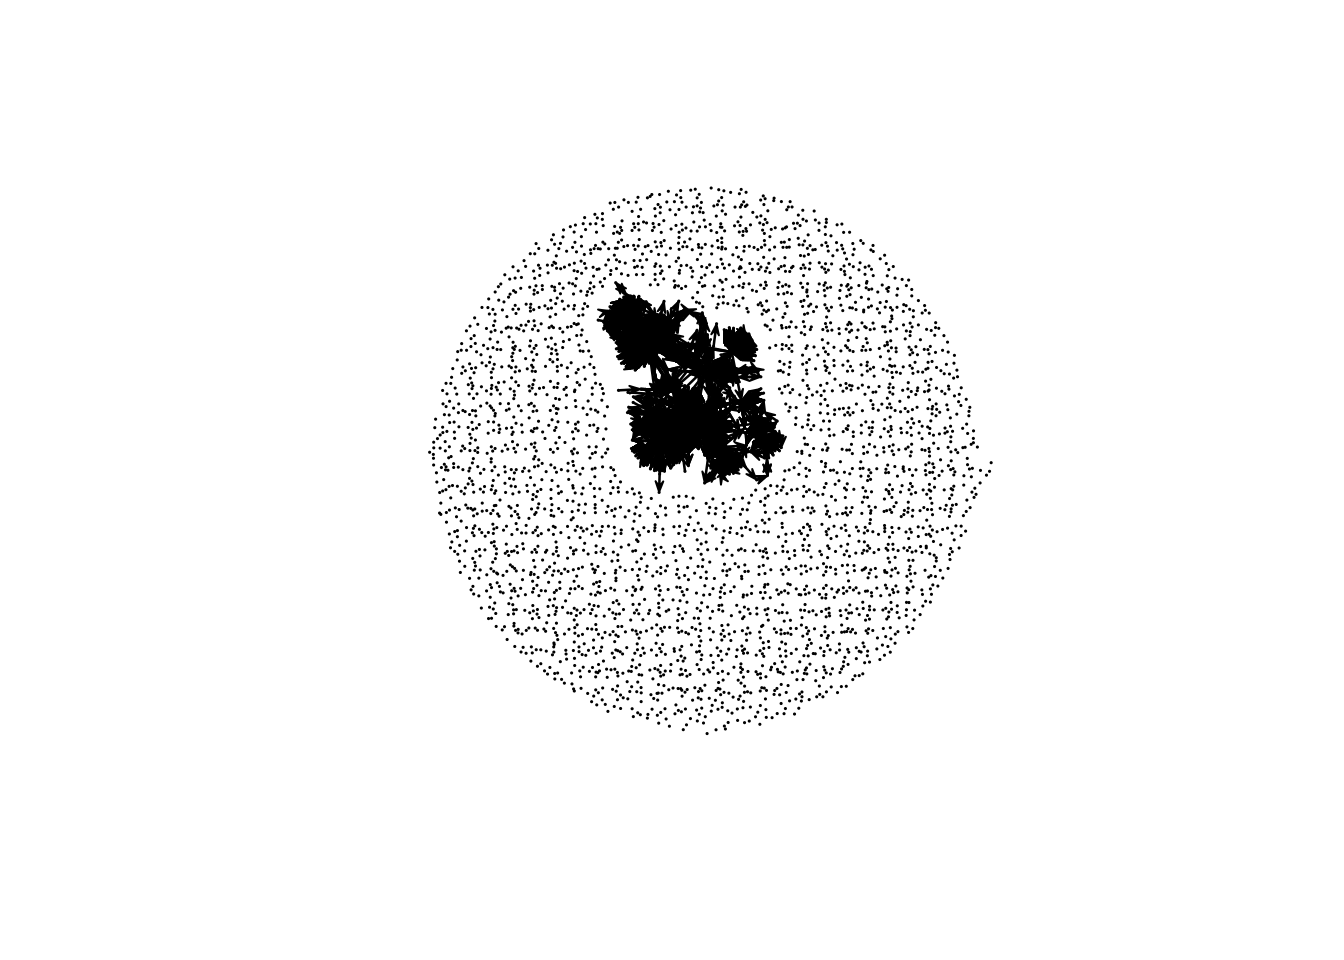
\includegraphics{graph_files/figure-latex/p_raw-1.pdf}

The graph shows a dense cluster of users with a high concentration of
potentially connected gropus of mutually interacting pairs surrounded by
a cloud of low interactivity.

\hypertarget{size}{%
\paragraph{Size}\label{size}}

\begin{Shaded}
\begin{Highlighting}[]
\NormalTok{net_raw}
\end{Highlighting}
\end{Shaded}

\begin{verbatim}
##  Network attributes:
##   vertices = 3660 
##   directed = TRUE 
##   hyper = FALSE 
##   loops = FALSE 
##   multiple = FALSE 
##   bipartite = FALSE 
##   total edges= 5268 
##     missing edges= 0 
##     non-missing edges= 5268 
## 
##  Vertex attribute names: 
##     vertex.names 
## 
##  Edge attribute names not shown
\end{verbatim}

\begin{Shaded}
\begin{Highlighting}[]
\NormalTok{raw_edges <-}\StringTok{  }\KeywordTok{length}\NormalTok{(net_raw}\OperatorTok{$}\NormalTok{mel)}
\NormalTok{raw_vertices <-}\StringTok{ }\NormalTok{net_raw}\OperatorTok{$}\NormalTok{gal}\OperatorTok{$}\NormalTok{n}
\end{Highlighting}
\end{Shaded}

The graph consists of \texttt{r} raw\_edges` edges, each representing
one or more emails, an average of 1.4393443 emails per user.

\hypertarget{density}{%
\paragraph{Density}\label{density}}

The graph has a density of 3.9337094\times 10\^{}\{-4\}, which is very
low.

\hypertarget{components}{%
\paragraph{Components}\label{components}}

As seen in the visualization of the graph, two components are present,
one that is strongly connected, and the other, weakly, comprising 3257
and 3196 members, respectively.

\hypertarget{diameter}{%
\paragraph{Diameter}\label{diameter}}

The diameter of the graph, 12, is the number of steps required to
connect the two nodes furthest apart.

\hypertarget{clustering}{%
\paragraph{Clustering}\label{clustering}}

The clustering coefficient of the graph is low, 0.0392917, indicating
relatively few users who belong to interacting groups.

\hypertarget{description-of-the-reduced-enron-graph}{%
\subsubsection{Description of the reduced Enron
graph}\label{description-of-the-reduced-enron-graph}}

Eliminating isolates reduces the number of connection endpoints from
5268 to 465. Within the original graph, the number of isolated node
pairs, those that do not connect to the dense cluster in the center, can
be eliminated to show the most interactive exchanges, thusly

\begin{verbatim}
net <- delete.vertices(net_raw, isolates(net_raw))
\end{verbatim}

\hypertarget{visualization-1}{%
\paragraph{Visualization}\label{visualization-1}}

The contrast between the original and reduced graph (after removing
isolates) is visually striking. Note that the edge line \emph{length}
does have any meaning; they vary solely to promote better visual
discrimination.

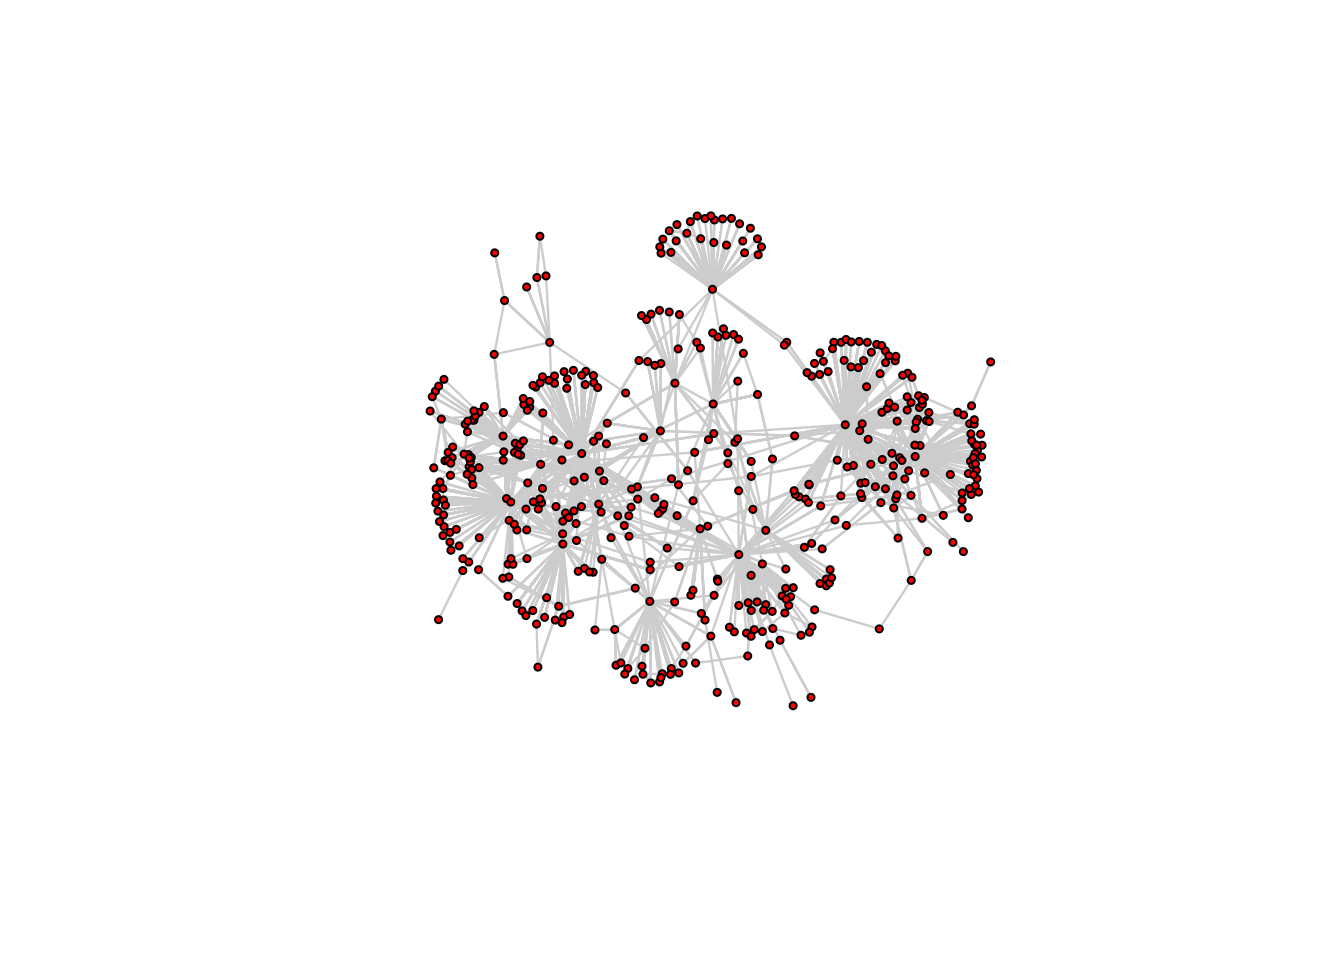
\includegraphics{graph_files/figure-latex/p-1.pdf}

The reduced graph is the dense portion of the original, but some more
readily discernable structure is apparent.

\hypertarget{density-1}{%
\paragraph{Density}\label{density-1}}

The graph has a density of 0.024416, compared to the original graph,
3.9337094\times 10\^{}\{-4\} or 62.0686874 greater.

\hypertarget{components-1}{%
\paragraph{Components}\label{components-1}}

As seen in the visualization of the graph, only 1 member is weakly
connected.

\hypertarget{diameter-1}{%
\paragraph{Diameter}\label{diameter-1}}

The diameter of the graph, 12, the number of steps required to connect
the two nodes furthest apart, is unchanged from the original.

\hypertarget{clustering-1}{%
\paragraph{Clustering}\label{clustering-1}}

The clustering coefficient of the graph is low, 0.0392917, essentially
identical to the original graph, indicating relatively few users who
belong to interacting groups.

\hypertarget{decomposition-of-the-reduced-enron-graph}{%
\subsubsection{Decomposition of the reduced Enron
graph}\label{decomposition-of-the-reduced-enron-graph}}

Among the nodes represented in the visualization above, some have
satellite nodes that connect principally to these center points. As a
reminder, the length of the edge lines carries no meaning, nor the
distance or proximity between dense portions of the graph. The rendering
algorithm's principal purpose is to spread out the links to promote
visual clarity.

Although, visual inspection shows some \emph{remote} nodes, every node
is directly or indirectly connected to every other node in the graph,
the number of isoletes is . However, visual inspection also shows that
\emph{some} nodes are much more connected than others.

To identify these, measures of \textbf{centrality}. Three of those are
\texttt{degree}, which measures aspects of the prominence of a node
(user) in the network based on how many or few intermediates are
required to reach any other node. The metric \texttt{betweenedness}
representes how many connections between other nodes must pass through
it to indirectly connect to nodes to which they are not directly
connected. The third measure \texttt{infocent} measures the directness
of a node to other nodes. Other measures of centrality exist, but the
scope of this paper excludes a comparison among them.

Instead, the three were measured for each node in the reduced graph,
giving them equal weight. The top 10\% of nodes with high
\texttt{degree} scores were selected, followed among those by the top
10\% of high \texttt{betweenedness} scores, then high \texttt{infocent}
scores to create a composite centrality indicator. Subsequent
adjustments may improve the efficacy of the machine learning approach in
this paper.

\begin{Shaded}
\begin{Highlighting}[]
\KeywordTok{load}\NormalTok{(}\StringTok{"prominence.Rda"}\NormalTok{)}
\NormalTok{prominence }\OperatorTok\StringTok{ }\KeywordTok{select}\NormalTok{(deg, btw, inf) }\OperatorTok\StringTok{ }\KeywordTok{cor}\NormalTok{()}
\end{Highlighting}
\end{Shaded}

\begin{verbatim}
##           deg       btw       inf
## deg 1.0000000 0.4670800 0.4799712
## btw 0.4670800 1.0000000 0.5591332
## inf 0.4799712 0.5591332 1.0000000
\end{verbatim}

\begin{Shaded}
\begin{Highlighting}[]
\NormalTok{prominence}
\end{Highlighting}
\end{Shaded}

\begin{verbatim}
## # A tibble: 16 x 8
##     name  node   deg    btw   inf pareto_deg pareto_btw pareto_inf
##    <int> <int> <dbl>  <dbl> <dbl>      <dbl>      <dbl>      <dbl>
##  1    25  1648    65 14624.  1.32      0.946      0.969      0.996
##  2    47  1717   130  3057.  1.11      0.969      0.912      0.962
##  3    62  1790    76 19095.  1.21      0.951      0.980      0.978
##  4   119  2055    52  8640.  1.20      0.930      0.951      0.975
##  5   149  2168    46 14787.  1.09      0.924      0.971      0.960
##  6   152  2191   170 15536.  1.29      0.978      0.973      0.987
##  7   174  2276   480 19518.  1.32      0.989      0.982      0.993
##  8   186  2310   216  9992.  1.31      0.982      0.957      0.989
##  9   236  2575  1439  3538.  1.26      1.000      0.917      0.982
## 10   237  2576   859 77161.  1.31      0.993      0.998      0.991
## 11   300  2946    38  6258.  1.02      0.917      0.939      0.910
## 12   347  3146  1009 86520.  1.35      0.998      1.000      1.000
## 13   349  3152    84 10121.  1.07      0.953      0.962      0.946
## 14   374  3250    65 34146.  1.25      0.946      0.993      0.980
## 15   375  3255   429 54562.  1.34      0.987      0.996      0.998
## 16   404  3421   577 33634.  1.28      0.991      0.991      0.984
\end{verbatim}

The three measures of prominence are correlated, to varying degrees,
indicating that they are measuring the characteristic of centrality
non-independently. Just 16 nodes are in the top 10\% of centrality.

\begin{Shaded}
\begin{Highlighting}[]
\KeywordTok{load}\NormalTok{(}\StringTok{"centrals.Rda"}\NormalTok{)}
\NormalTok{net_p <-}\StringTok{ }\KeywordTok{network}\NormalTok{(prominence, }\DataTypeTok{matrix.type =} \StringTok{"edgelist"}\NormalTok{)}
\NormalTok{vertices <-}\StringTok{ }\KeywordTok{network.vertex.names}\NormalTok{(net_p)}
\NormalTok{prominent <-}\StringTok{ }\NormalTok{g_enron }\OperatorTok\StringTok{ }\KeywordTok{filter}\NormalTok{(f_userid }\OperatorTok\StringTok{ }\NormalTok{centrals }\OperatorTok{|}\StringTok{ }\NormalTok{t_userid }\OperatorTok\StringTok{ }\NormalTok{centrals)}
\end{Highlighting}
\end{Shaded}

These 16 users are connected to 3405 other users. They account for
90.4517844\% of the emails, as sender or receiver, in the reduced graph.
Limiting the reduced graph to these central users results in the
following graph.

\begin{Shaded}
\begin{Highlighting}[]
\KeywordTok{load}\NormalTok{(}\StringTok{"prominent.Rda"}\NormalTok{)}
\NormalTok{netmat <-}\StringTok{ }\NormalTok{prominent }\OperatorTok\StringTok{ }\KeywordTok{select}\NormalTok{(t_userid, f_userid)}
\NormalTok{net_p <-}\StringTok{ }\KeywordTok{network}\NormalTok{(netmat, }\DataTypeTok{matrix.type =} \StringTok{"edgelist"}\NormalTok{)}
\NormalTok{vertices <-}\StringTok{ }\KeywordTok{network.vertex.names}\NormalTok{(net_p)}
\KeywordTok{ggnet}\NormalTok{(net_p, }\DataTypeTok{size =} \FloatTok{0.1}\NormalTok{, }\DataTypeTok{alpha =} \FloatTok{0.84}\NormalTok{)}
\end{Highlighting}
\end{Shaded}

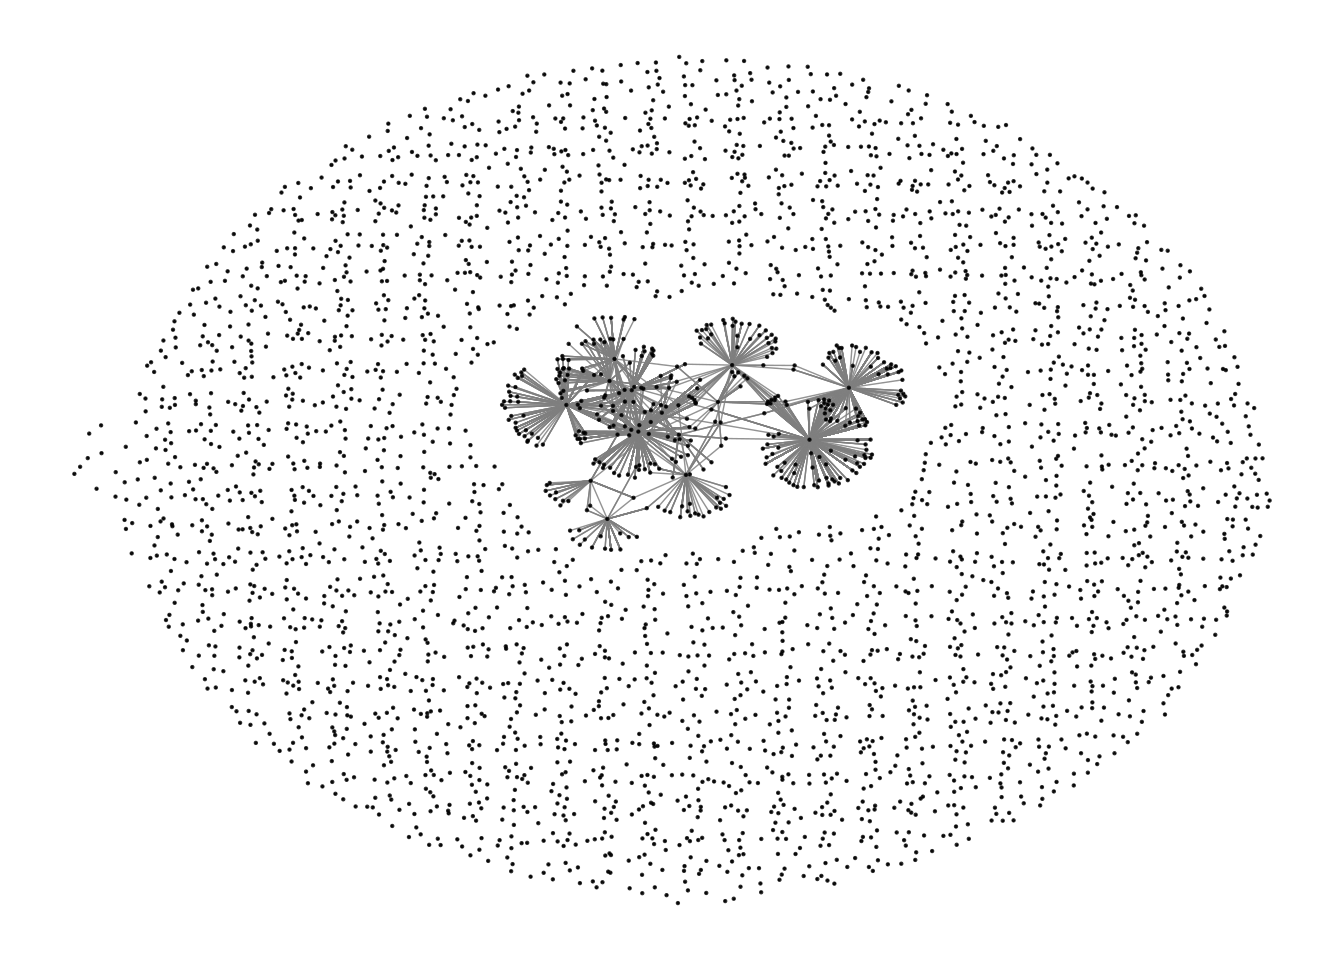
\includegraphics{graph_files/figure-latex/unnamed-chunk-2-1.pdf}

This visualization, like original graph, shows ``noise'' in the form of
a cloud of poorly connected node pairs surrounding a denser inner core,
even after senders and receivers were restricted to the most prominent
users.

\begin{Shaded}
\begin{Highlighting}[]
\NormalTok{net_p}
\end{Highlighting}
\end{Shaded}

\begin{verbatim}
##  Network attributes:
##   vertices = 3660 
##   directed = TRUE 
##   hyper = FALSE 
##   loops = FALSE 
##   multiple = FALSE 
##   bipartite = FALSE 
##   total edges= 4765 
##     missing edges= 0 
##     non-missing edges= 4765 
## 
##  Vertex attribute names: 
##     vertex.names 
## 
##  Edge attribute names not shown
\end{verbatim}

\begin{Shaded}
\begin{Highlighting}[]
\NormalTok{vertices_before <-}\StringTok{ }\KeywordTok{length}\NormalTok{(}\KeywordTok{network.vertex.names}\NormalTok{(net_p))}
\end{Highlighting}
\end{Shaded}

\begin{Shaded}
\begin{Highlighting}[]
\KeywordTok{delete.vertices}\NormalTok{(net_p, }\KeywordTok{isolates}\NormalTok{(net_p))}
\NormalTok{vertices_after <-}\StringTok{ }\KeywordTok{length}\NormalTok{(}\KeywordTok{network.vertex.names}\NormalTok{(net_p))}
\KeywordTok{ggnet}\NormalTok{(net_p, }\DataTypeTok{size =} \FloatTok{0.1}\NormalTok{, }\DataTypeTok{alpha =} \FloatTok{0.84}\NormalTok{)}
\end{Highlighting}
\end{Shaded}

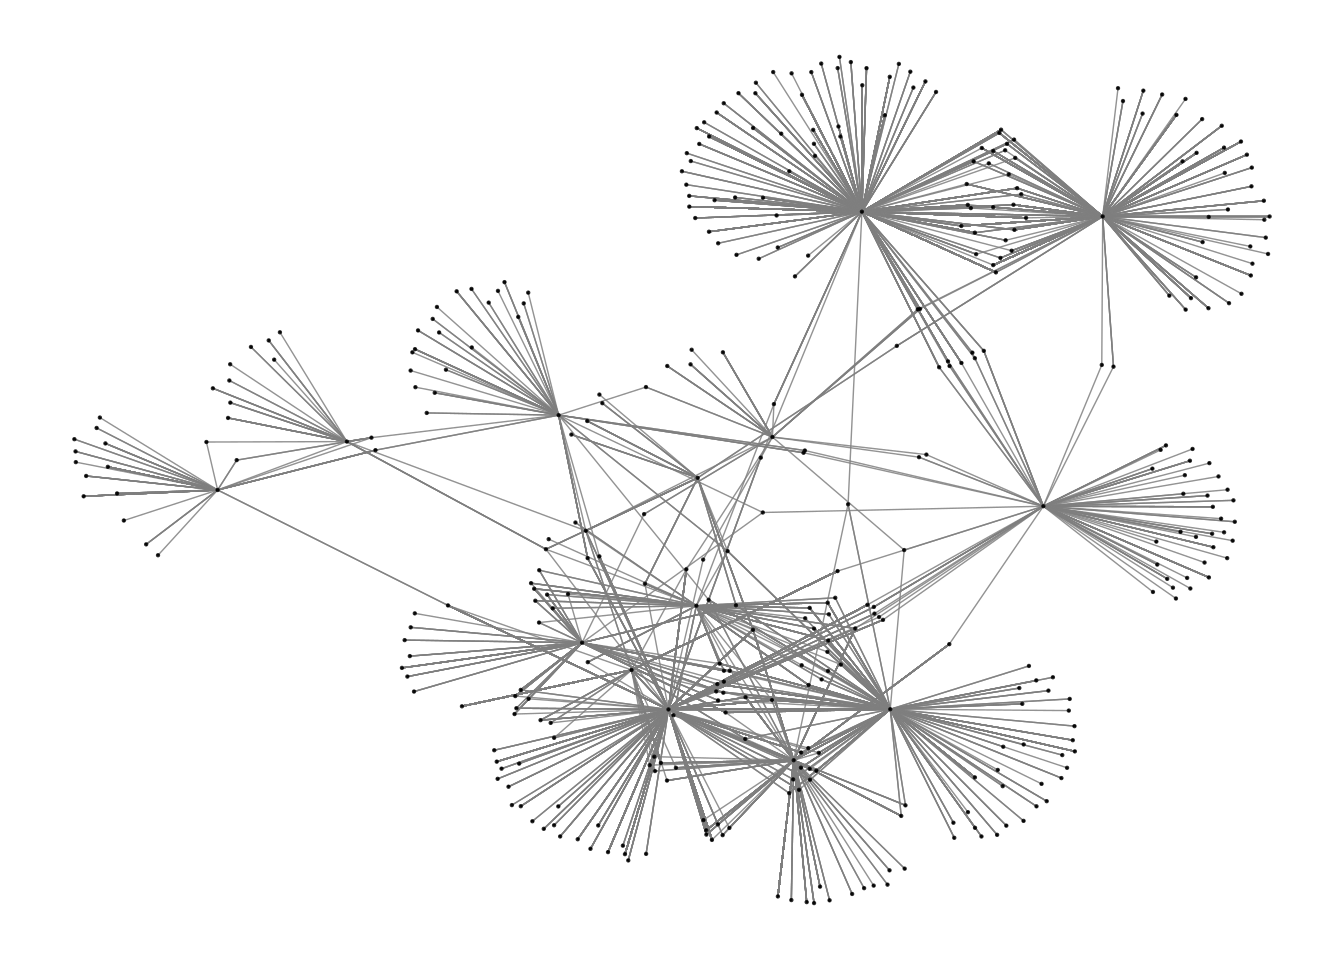
\includegraphics{graph_files/figure-latex/unnamed-chunk-4-1.pdf}

Removing those outliers brings the core network into sharper relief by
reducing the number of vertices, from 3660 to 399.

\hypertarget{machine-learning-decomposition-of-the-core-network}{%
\subsubsection{Machine learning decomposition of the core
network}\label{machine-learning-decomposition-of-the-core-network}}

Although the network has been reduced by inspection, the visualization
of the result is ambiguous as to clusters of similar senders/recievers
(nodes/edges). To validate the results, a machine learning tool is
indicated. The {[}latentnet{]} package was selected for that task. An
{[}accessible{]} description of that package, as well as a more
{[}theoretical{]} paper are available for orientation.

The package applies exponential random graph modeling to the vertices,
edges and optionally their attrtibutes to recursively dervive graph
characteristics that are impractical to extract otherwise, due to the
interdependence of graph measures.

\hypertarget{model-creation}{%
\paragraph{Model creation}\label{model-creation}}

The first step is to fit a model to a network object:

\begin{verbatim}
  net_p.fit <- ergmm(net_p ~ euclidean(d=2, G=3), verbose = TRUE) # up to 30 minutes for 250 nodes
  Generating initial values for MCMC:
  Computing geodesic distances... Finished.
  Computing MDS locations... Finished.
  Computing other initial values... Finished.
  Finding the conditional posterior mode... Finished.
  Burning in... Finished.
  Starting sampling run... Finished.
  Post-processing the MCMC output:
  Performing label-switching... Finished.
  Fitting the MKL locations... Finished.
  Fitting MBC conditional on MKL locations... Finished.
\end{verbatim}

The arguments to \texttt{ergmm} specify a negative Euclidian distance in
2-space for a three cluster grouping. The algorithm performs a Markov
chain Monte Carlo simulation, the absolute row/column differences within
the adjacency matrix to fit the Minimum Kullback-Liebler divergence
statistic to produce model based clustering of the vertices in the
graph.

\begin{Shaded}
\begin{Highlighting}[]
\KeywordTok{library}\NormalTok{(latentnet)}
\KeywordTok{library}\NormalTok{(coda)}
\KeywordTok{load}\NormalTok{(}\StringTok{"net_p.fit.Rda"}\NormalTok{)}
\KeywordTok{summary}\NormalTok{(net_p.fit)}
\end{Highlighting}
\end{Shaded}

\begin{verbatim}
## NOTE: It is not certain whether it is appropriate to use latentnet's BIC to select latent space dimension, whether or not to include actor-specific random effects, and to compare clustered models with the unclustered model.
\end{verbatim}

\begin{verbatim}
## 
## ==========================
## Summary of model fit
## ==========================
## 
## Formula:   net_p ~ euclidean(d = 2, G = 3)
## Attribute: edges
## Model:     Bernoulli 
## MCMC sample of size 4000, draws are 10 iterations apart, after burnin of 10000 iterations.
## Covariate coefficients posterior means:
##             Estimate    2.5%   97.5% 2*min(Pr(>0),Pr(<0))    
## (Intercept)  -1.9744 -2.1183 -1.8386            < 2.2e-16 ***
## ---
## Signif. codes:  0 '***' 0.001 '**' 0.01 '*' 0.05 '.' 0.1 ' ' 1
## 
## Overall BIC:        10914.77 
## Likelihood BIC:     8384.658 
## Latent space/clustering BIC:     2530.115 
## 
## Covariate coefficients MKL:
##              Estimate
## (Intercept) -3.315879
\end{verbatim}

\begin{figure}
\centering
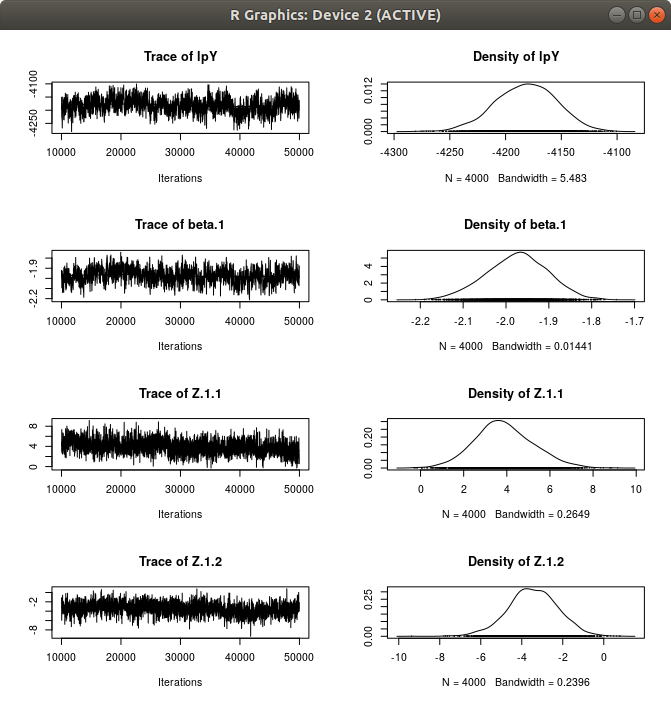
\includegraphics{net_p.fit_trace.png}
\caption{Trace diagnostic of net\_p.fit}
\end{figure}

\hypertarget{model-diagnostics}{%
\paragraph{Model Diagnostics}\label{model-diagnostics}}

Graphs do not uniformly converge under the \texttt{ergmm} function call.
To test this, a diagnostic is available to detect failure of the Markov
chain Monte Carlo simulation to converge and to detect autocorrelation
effects. One section provides an initial and lag 10 covariance matrix of
the sampling.

\begin{Shaded}
\begin{Highlighting}[]
\KeywordTok{load}\NormalTok{(}\StringTok{"net_p.fit.Rda"}\NormalTok{)}
\KeywordTok{mcmc.diagnostics}\NormalTok{(net_p.fit, }\DataTypeTok{which.diags =} \KeywordTok{c}\NormalTok{(}\StringTok{"cor"}\NormalTok{, }\StringTok{"acf"}\NormalTok{, }\StringTok{"rafferty"}\NormalTok{))}
\end{Highlighting}
\end{Shaded}

\begin{verbatim}
## Chain 1 
## Lag 0 
##               lpY      beta.1       Z.1.1       Z.1.2
## lpY    1.00000000  0.47541395  0.04536734  0.01857208
## beta.1 0.47541395  1.00000000  0.06473074 -0.05372611
## Z.1.1  0.04536734  0.06473074  1.00000000 -0.01356222
## Z.1.2  0.01857208 -0.05372611 -0.01356222  1.00000000
## 
## Lag 10 
##               lpY      beta.1      Z.1.1       Z.1.2
## lpY    0.60827334  0.43742187 0.04284890  0.01703367
## beta.1 0.44226482  0.71444735 0.04422307 -0.03119275
## Z.1.1  0.03936699  0.05665058 0.28978163  0.01203623
## Z.1.2  0.01927168 -0.02159930 0.02894825  0.24651351
\end{verbatim}

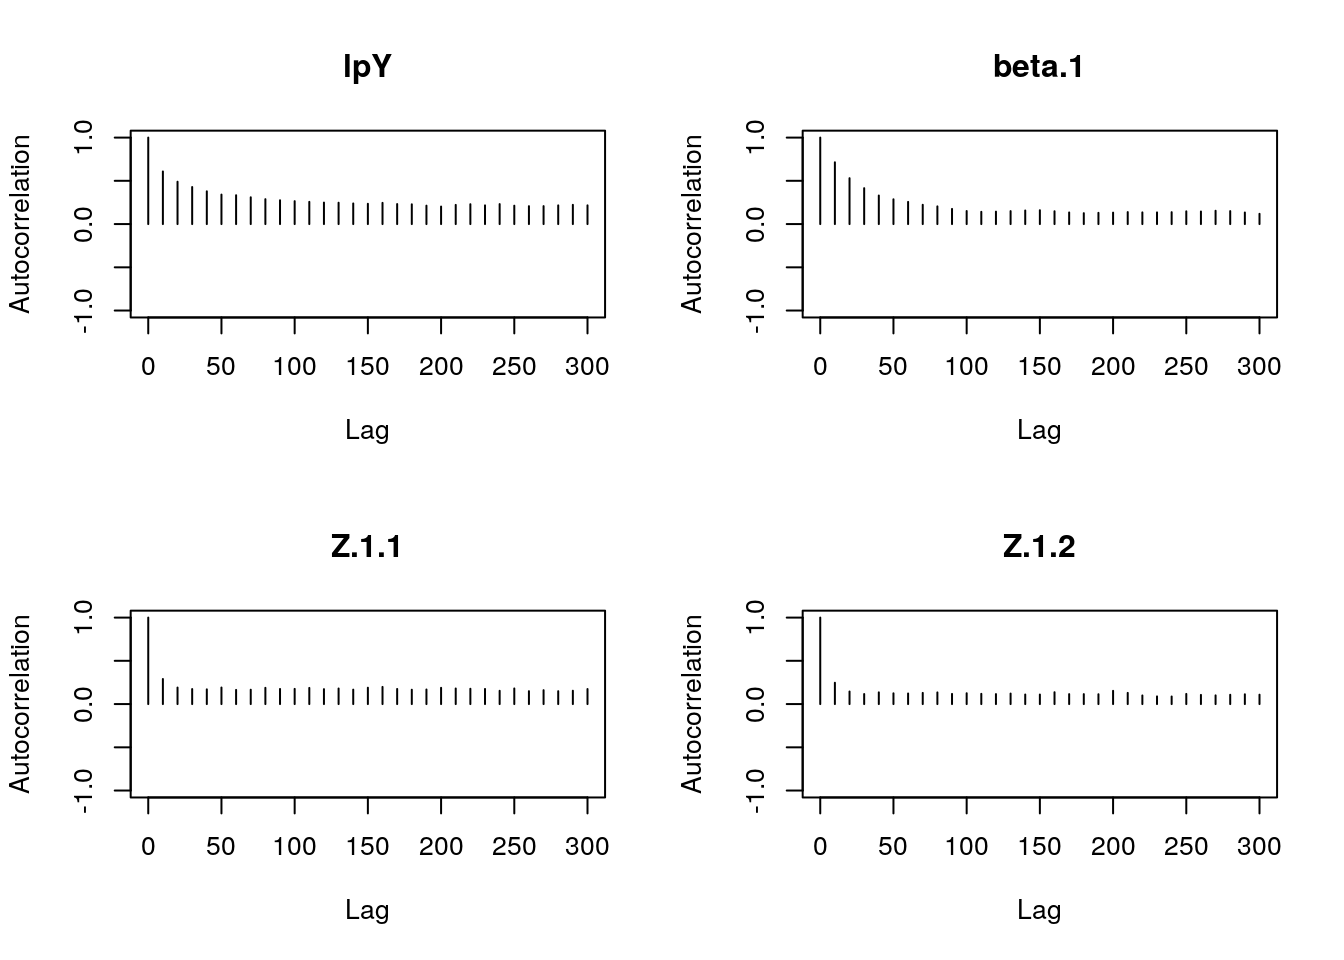
\includegraphics{graph_files/figure-latex/unnamed-chunk-6-1.pdf}

\hypertarget{goodness-of-fit}{%
\paragraph{Goodness of fit}\label{goodness-of-fit}}

\begin{Shaded}
\begin{Highlighting}[]
\NormalTok{net_p.gof <-}\StringTok{ }\KeywordTok{gof}\NormalTok{(net_p.fit)}
\NormalTok{net_p.gof}
\end{Highlighting}
\end{Shaded}

\begin{verbatim}
## 
## Goodness-of-fit for in-degree 
## 
##    obs min  mean max MC p-value
## 0   43  47 63.33  85       0.00
## 1  276  70 95.72 121       0.00
## 2   59  71 91.86 117       0.00
## 3    5  47 68.19  93       0.00
## 4    2  30 40.84  55       0.00
## 5    1  10 22.04  36       0.00
## 6    0   1 10.42  17       0.00
## 7    0   0  4.38   9       0.06
## 8    0   0  1.43   5       0.64
## 9    1   0  0.49   3       0.78
## 10   1   0  0.21   2       0.40
## 11   0   0  0.04   1       1.00
## 12   1   0  0.05   1       0.10
## 14   1   0  0.00   0       0.00
## 15   1   0  0.00   0       0.00
## 17   1   0  0.00   0       0.00
## 26   1   0  0.00   0       0.00
## 36   2   0  0.00   0       0.00
## 61   1   0  0.00   0       0.00
## 63   1   0  0.00   0       0.00
## 69   1   0  0.00   0       0.00
## 83   1   0  0.00   0       0.00
## 
## Goodness-of-fit for out-degree 
## 
##    obs min  mean max MC p-value
## 0   56  45 63.30  84       0.34
## 1  234  71 96.81 125       0.00
## 2   81  69 89.87 110       0.30
## 3   12  53 68.50  88       0.00
## 4    3  26 41.12  59       0.00
## 5    0   9 22.53  37       0.00
## 6    2   3 10.67  24       0.00
## 7    0   0  3.91  11       0.08
## 8    0   0  1.68   5       0.44
## 9    0   0  0.42   3       1.00
## 10   0   0  0.15   2       1.00
## 11   1   0  0.03   1       0.06
## 12   1   0  0.01   1       0.02
## 15   1   0  0.00   0       0.00
## 27   2   0  0.00   0       0.00
## 33   1   0  0.00   0       0.00
## 50   1   0  0.00   0       0.00
## 55   2   0  0.00   0       0.00
## 57   1   0  0.00   0       0.00
## 75   1   0  0.00   0       0.00
## 
## Goodness-of-fit for minimum geodesic distance 
## 
##       obs   min     mean   max MC p-value
## 1     873   783   869.74   996       0.90
## 2   18656  1682  2042.89  2704       0.00
## 3   15596  3361  4401.85  6373       0.00
## 4   25842  5365  7669.38 11461       0.00
## 5   12184  6753 10251.28 14754       0.18
## 6   14434  7166 11054.85 16742       0.06
## 7   10916  6266 10741.51 17232       0.96
## 8    3020  4704 10173.04 15597       0.00
## 9    2128  3941  9451.88 13642       0.00
## 10      0  3731  8289.79 11629       0.00
## 11      0  3421  6641.97  9005       0.00
## 12      0  1618  4836.98  7948       0.00
## 13      0   690  3255.56  6973       0.00
## 14      0   262  2072.12  6193       0.00
## 15      0   105  1264.45  4808       0.00
## 16      0    23   749.52  3257       0.00
## 17      0     5   441.22  3000       0.00
## 18      0     0   259.06  2787       0.04
## 19      0     0   153.04  2234       0.18
## 20      0     0    89.17  1423       0.44
## 21      0     0    50.37   722       0.88
## 22      0     0    26.81   456       1.00
## 23      0     0    12.96   297       1.00
## 24      0     0     5.95   154       1.00
## 25      0     0     2.30    56       1.00
## 26      0     0     0.68    20       1.00
## 27      0     0     0.15     4       1.00
## 28      0     0     0.02     1       1.00
## Inf 55153 48239 63993.46 92771       0.18
\end{verbatim}

\begin{Shaded}
\begin{Highlighting}[]
\KeywordTok{par}\NormalTok{(}\DataTypeTok{mfrow=}\KeywordTok{c}\NormalTok{(}\DecValTok{1}\NormalTok{,}\DecValTok{3}\NormalTok{))}
\KeywordTok{par}\NormalTok{(}\DataTypeTok{oma=}\KeywordTok{c}\NormalTok{(}\FloatTok{0.5}\NormalTok{,}\DecValTok{2}\NormalTok{,}\DecValTok{1}\NormalTok{,}\FloatTok{0.5}\NormalTok{))}
\KeywordTok{plot}\NormalTok{(net_p.gof, }\DataTypeTok{plotlogodds=}\OtherTok{TRUE}\NormalTok{)}
\end{Highlighting}
\end{Shaded}

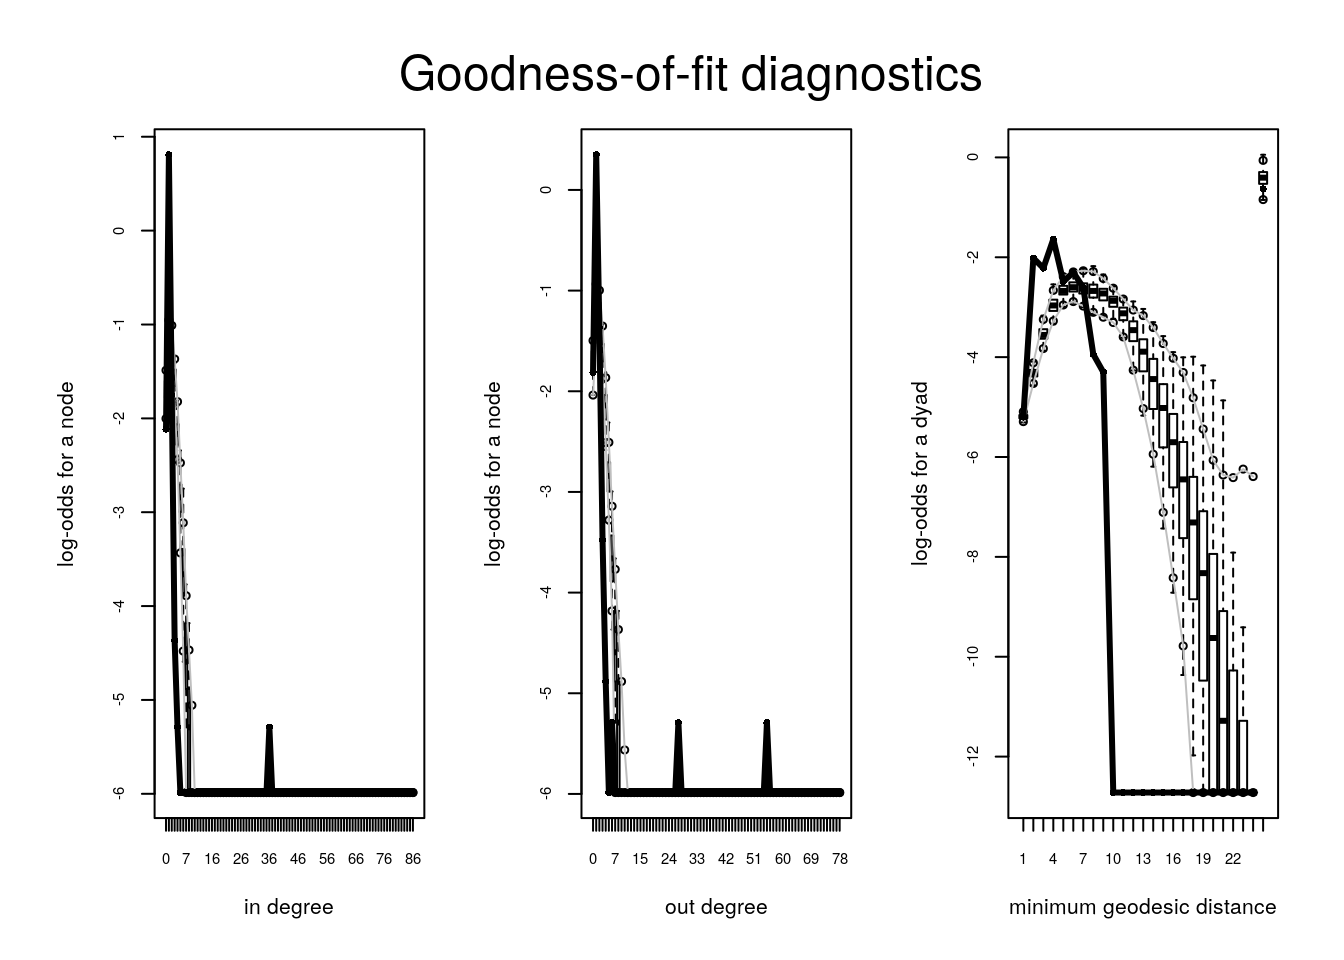
\includegraphics{graph_files/figure-latex/unnamed-chunk-7-1.pdf}

\hypertarget{visualization-of-model-clusters-position-within-sample-space-and-density}{%
\paragraph{Visualization of model clusters, position within sample space
and
density}\label{visualization-of-model-clusters-position-within-sample-space-and-density}}

\begin{Shaded}
\begin{Highlighting}[]
\KeywordTok{plot}\NormalTok{(net_p.fit, }\DataTypeTok{pie=}\OtherTok{TRUE}\NormalTok{)}
\end{Highlighting}
\end{Shaded}

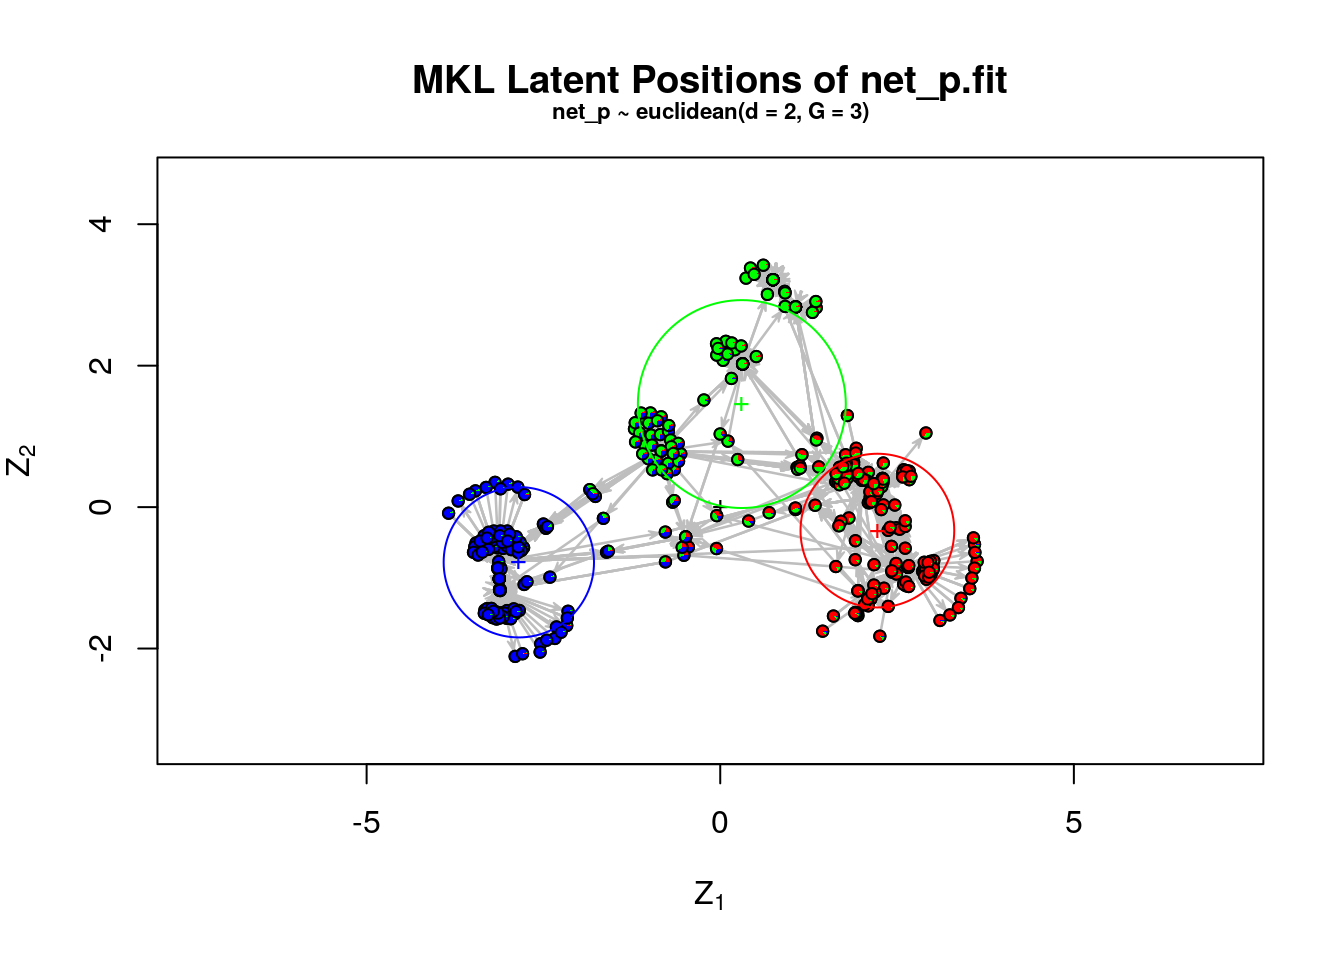
\includegraphics{graph_files/figure-latex/unnamed-chunk-8-1.pdf}

\begin{Shaded}
\begin{Highlighting}[]
\KeywordTok{plot}\NormalTok{(net_p.fit, }\DataTypeTok{what=}\StringTok{"cloud"}\NormalTok{, }\DataTypeTok{rand.eff=}\StringTok{"receiver"}\NormalTok{, }\DataTypeTok{Z.ref=}\NormalTok{Z.ref, }\DataTypeTok{Z.K.ref=}\NormalTok{Z.K.ref)}
\end{Highlighting}
\end{Shaded}

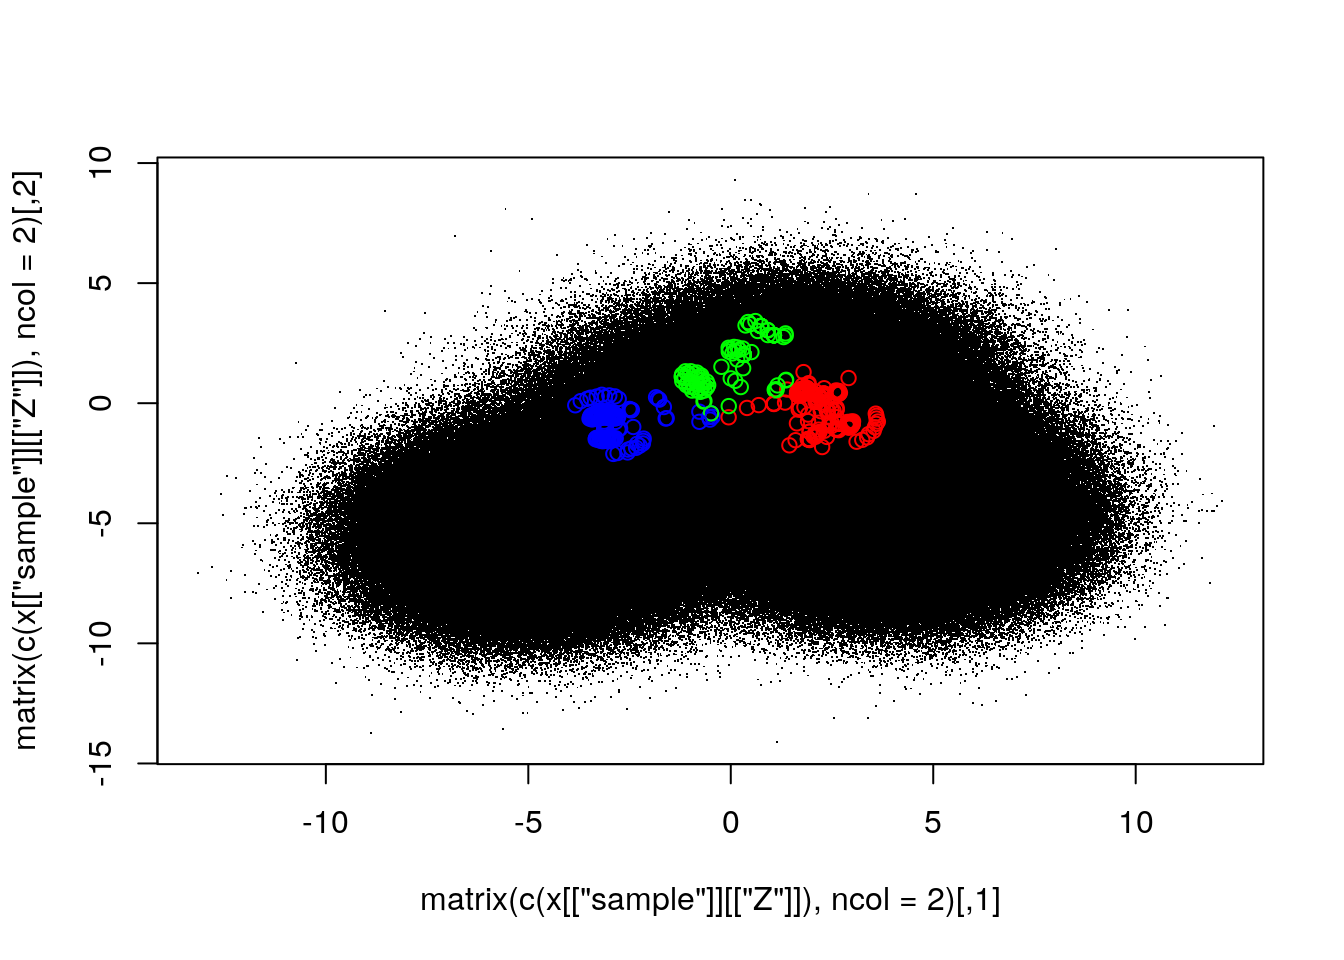
\includegraphics{graph_files/figure-latex/unnamed-chunk-8-2.pdf}

\begin{Shaded}
\begin{Highlighting}[]
\KeywordTok{plot}\NormalTok{(net_p.fit, }\DataTypeTok{what=}\StringTok{"density"}\NormalTok{, }\DataTypeTok{rand.eff=}\StringTok{"receiver"}\NormalTok{, }\DataTypeTok{Z.ref=}\NormalTok{Z.ref, }\DataTypeTok{Z.K.ref=}\NormalTok{Z.K.ref)}
\end{Highlighting}
\end{Shaded}

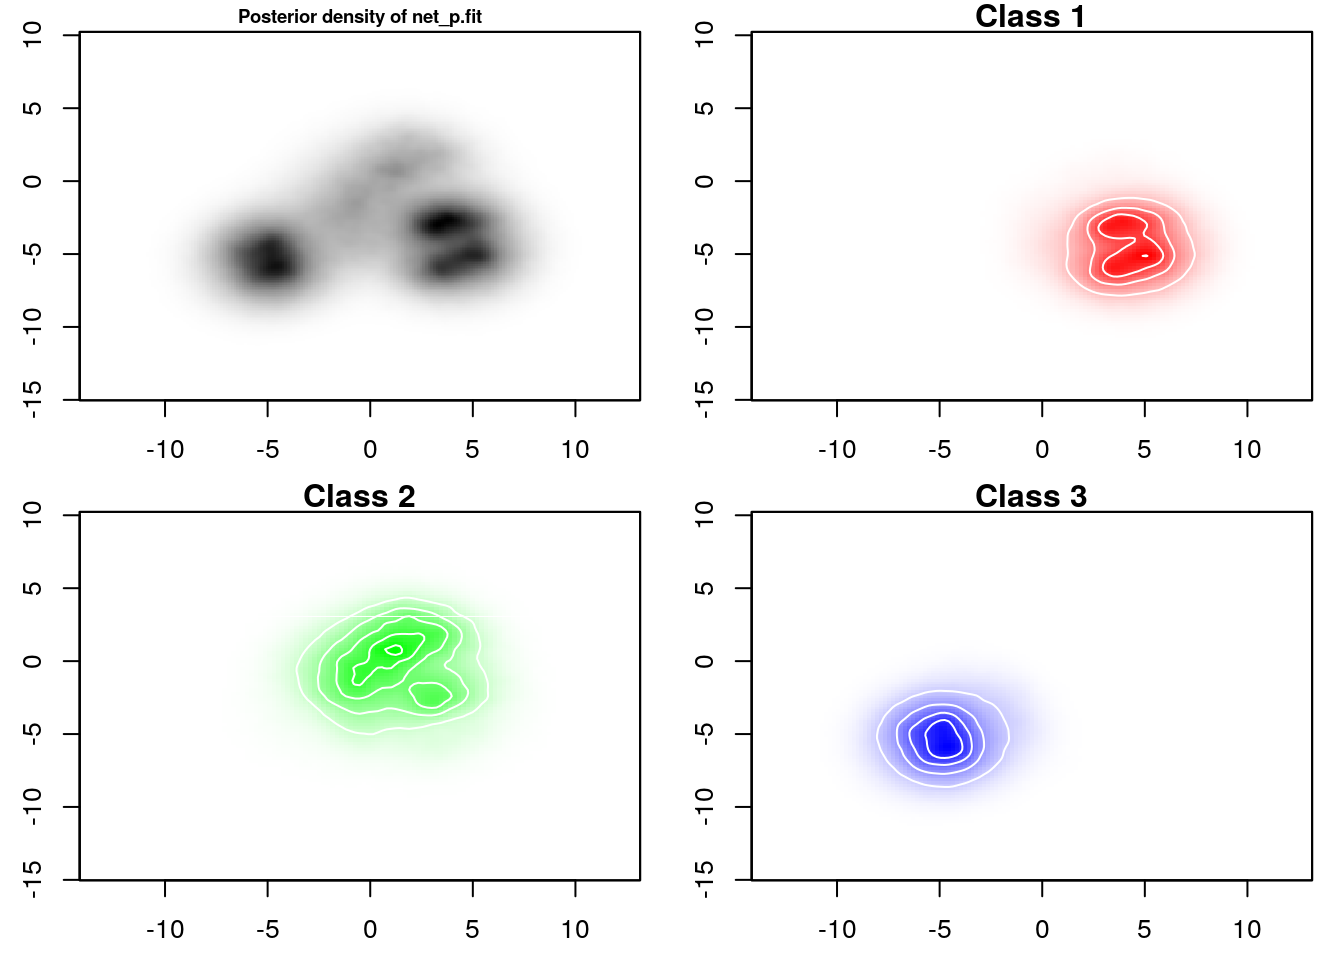
\includegraphics{graph_files/figure-latex/unnamed-chunk-8-3.pdf}

Using the cluster assignment to sender and recipient userids confirms
the graph:

\begin{Shaded}
\begin{Highlighting}[]
\KeywordTok{load}\NormalTok{(}\StringTok{"n_enron.Rda"}\NormalTok{)}
\NormalTok{n_enron }\OperatorTok\StringTok{ }\KeywordTok{group_by}\NormalTok{(f_cluster, t_cluster) }\OperatorTok\StringTok{ }\KeywordTok{count}\NormalTok{() }\OperatorTok\StringTok{ }\KeywordTok{arrange}\NormalTok{(}\KeywordTok{desc}\NormalTok{(n))}
\end{Highlighting}
\end{Shaded}

\begin{verbatim}
## # A tibble: 8 x 3
## # Groups:   f_cluster, t_cluster [8]
##   f_cluster t_cluster     n
##       <int>     <int> <int>
## 1         1         1  1913
## 2         3         3  1315
## 3         1         2   547
## 4         2         1   541
## 5         2         2   387
## 6         3         2    41
## 7         2         3    20
## 8         1         3     1
\end{verbatim}

Members of cluster 1 correspond predominantly to other members of
cluster 1 and to a substantial number of cluster 2 members. There is
only one message from a cluster 1 member to a cluster 3 member. Cluster
2 members have an even division of emails sent to or received from
cluster 1 and a smaller cluster 2 to cluster 2 correspondence.
Correspondence between clusters 2 and 3, in either direction, is much
less.

\hypertarget{application-of-the-deconstruction-of-the-enron-network}{%
\paragraph{Application of the deconstruction of the Enron
network}\label{application-of-the-deconstruction-of-the-enron-network}}

Through a combination of analytic judgment and machine learning a
three-cluster partition of the emails has been created. The obvious
question to now be addressed is what those clusters represent in terms
of email content. For that the tools of natural language processing will
be applied.


\end{document}
